\documentclass[12pt]{article}
\usepackage{latexblog}

% ============================================================
% Blog Metadata
% ============================================================
\blogtitle{搭建Openshift本地环境}
\blogdate{2020-03-09}
\blogtags{Docker, OpenShift, 云计算, 容器化}
\bloglang{zh}
\blogsummary{}

\begin{document}
\makeblogtitle

OpenShift是红帽基于Docker和Kubernetes的云开发平台即服务（PaaS）。而\href{https://www.okd.io/}{OKD(The Origin Community Distribution of Kubernetes )}即Openshift的开源版本。在本机上搭建一套完整的Openshift环境较为麻烦，有以下几种方式：

\begin{itemize}
\tightlist
\item
  Running in a Container
\item
  Run the All-In-One VM with Minishift
\item
  使用Virtualbox构建Openshift集群
\end{itemize}

\section{使用VirtualBox构建Openshift集群}\label{ux4f7fux7528virtualboxux6784ux5efaopenshiftux96c6ux7fa4}

按照\href{https://docs.openshift.com/container-platform/3.11/install/index.html}{安装文档}应该可以在本地搭建一个集群，但是纯手动安装的话比较复杂，幸好有\href{https://github.com/eliu/openshift-vagrant}{Openshift Vagrant}这个项目可以帮助我们简单的构建出一个集群环境。

\subsection{集群规划}\label{ux96c6ux7fa4ux89c4ux5212}

下面是计划搭建的最简单的单master、多node的一个集群配置：

{\def\LTcaptype{none} % do not increment counter
\begin{longtable}[]{@{}llll@{}}
\toprule\noalign{}
Node & IP & Role & Instance \\
\midrule\noalign{}
\endhead
\bottomrule\noalign{}
\endlastfoot
master.example.com & .100 & node, master, etcd & 4GMem, 2Core, 40GDisk \\
node1.example.com & .101 & node & 2GMem, 1Core, 40GDisk \\
node2.example.com & .102 & node & 2GMem, 1Core, 40GDisk \\
\end{longtable}
}

整个安装步骤可以分为这几步：

\begin{itemize}
\tightlist
\item
  创建好master、node三个虚拟机
\item
  通过hosts文件设置好域名解析
\item
  在master、node上都安装docker依赖
\item
  配置在master上可以通过ssh访问到node01、node02
\item
  在master上安装ansible
\item
  在master上执行openshift-ansible部署openshift
\end{itemize}

\subsection{定义虚拟机}\label{ux5b9aux4e49ux865aux62dfux673a}

如果手动从virtualbox安装虚拟机、再安装系统的话，需要耗费不少时间，通过Vagrant我们可以快速自动化地创建出这样的一个机器集群，类似从docker拉取image一样。定义这些只需要创建一个Vagrantfile：

\begin{Shaded}
\begin{Highlighting}[]
\VariableTok{Vagrant}\OperatorTok{.}\NormalTok{configure}\OperatorTok{(}\StringTok{"2"}\OperatorTok{)} \ControlFlowTok{do} \OperatorTok{|}\VariableTok{config}\OperatorTok{|}
    \VariableTok{config}\OperatorTok{.}\VariableTok{vm}\OperatorTok{.}\VariableTok{box} \OperatorTok{=} \StringTok{"centos/7"}
    \VariableTok{config}\OperatorTok{.}\VariableTok{vm}\OperatorTok{.}\VariableTok{box\_check\_update} \OperatorTok{=} \KeywordTok{false}

    \VariableTok{config}\OperatorTok{.}\VariableTok{vm}\OperatorTok{.}\NormalTok{provider }\StringTok{"virtualbox"} \ControlFlowTok{do} \OperatorTok{|}\VariableTok{vb}\OperatorTok{|}
        \VariableTok{vb}\OperatorTok{.}\VariableTok{memory} \OperatorTok{=} \DecValTok{2048}
        \VariableTok{vb}\OperatorTok{.}\VariableTok{cpus} \OperatorTok{=} \DecValTok{1}
    \ControlFlowTok{end}

    \VariableTok{config}\OperatorTok{.}\VariableTok{vm}\OperatorTok{.}\NormalTok{provision }\StringTok{"shell"}\OperatorTok{,} \VariableTok{inline}\OperatorTok{:} \OperatorTok{\textless{}\textless{}{-}}\ConstantTok{SHELL}
        \OperatorTok{/}\VariableTok{vagrant}\OperatorTok{/}\VariableTok{common}\OperatorTok{.}\VariableTok{sh}
    \ConstantTok{SHELL}

    \VariableTok{config}\OperatorTok{.}\VariableTok{hostmanager}\OperatorTok{.}\VariableTok{enabled} \OperatorTok{=} \KeywordTok{true}
    \VariableTok{config}\OperatorTok{.}\VariableTok{hostmanager}\OperatorTok{.}\VariableTok{manage\_host} \OperatorTok{=} \KeywordTok{true}
    \VariableTok{config}\OperatorTok{.}\VariableTok{hostmanager}\OperatorTok{.}\VariableTok{ignore\_private\_ip} \OperatorTok{=} \KeywordTok{false}
  
    \OperatorTok{(}\DecValTok{1..2}\OperatorTok{).}\VariableTok{each} \ControlFlowTok{do} \OperatorTok{|}\VariableTok{i}\OperatorTok{|}
        \VariableTok{config}\OperatorTok{.}\VariableTok{vm}\OperatorTok{.}\NormalTok{define }\StringTok{"node0\#\{i\}"} \ControlFlowTok{do} \OperatorTok{|}\VariableTok{node}\OperatorTok{|}
            \VariableTok{node}\OperatorTok{.}\VariableTok{vm}\OperatorTok{.}\NormalTok{network }\StringTok{"private\_network"}\OperatorTok{,} \VariableTok{ip}\OperatorTok{:} \StringTok{"\#\{NETWORK\_BASE\}\#\{i\}"}
            \VariableTok{node}\OperatorTok{.}\VariableTok{vm}\OperatorTok{.}\VariableTok{hostname} \OperatorTok{=} \StringTok{"node0\#\{i\}.example.com"}
        \ControlFlowTok{end}
    \ControlFlowTok{end}
\ControlFlowTok{end}
\end{Highlighting}
\end{Shaded}

以上的配置定义了操作系统、内存和cpu，以及网络和域名设置，然后创建node01、node02。这里用到了vagrant的hostmanager插件，他会去修改宿主机以及虚拟机的hosts文件，增加域名映射。同时，可以把一些公共的依赖项安装脚本进行provision，例如安装docker。然后，还需要创建master节点：

\begin{Shaded}
\begin{Highlighting}[]
\VariableTok{config}\OperatorTok{.}\VariableTok{vm}\OperatorTok{.}\NormalTok{define }\StringTok{"master"}\OperatorTok{,} \VariableTok{primary}\OperatorTok{:} \KeywordTok{true} \ControlFlowTok{do} \OperatorTok{|}\VariableTok{master}\OperatorTok{|}
        \VariableTok{master}\OperatorTok{.}\VariableTok{vm}\OperatorTok{.}\NormalTok{network }\StringTok{"private\_network"}\OperatorTok{,} \VariableTok{ip}\OperatorTok{:} \StringTok{"\#\{NETWORK\_BASE\}0"}
        \OperatorTok{\#} \VariableTok{master}\OperatorTok{.}\VariableTok{vm}\OperatorTok{.}\VariableTok{hostname} \OperatorTok{=} \StringTok{"master.example.com"}
        \VariableTok{master}\OperatorTok{.}\VariableTok{hostmanager}\OperatorTok{.}\VariableTok{aliases} \OperatorTok{=} \OperatorTok{\%}\NormalTok{w}\OperatorTok{(}\VariableTok{master}\OperatorTok{.}\VariableTok{example}\OperatorTok{.}\VariableTok{com} \VariableTok{etcd}\OperatorTok{.}\VariableTok{example}\OperatorTok{.}\VariableTok{com} \VariableTok{nfs}\OperatorTok{.}\VariableTok{example}\OperatorTok{.}\VariableTok{com}\OperatorTok{)}
        \VariableTok{master}\OperatorTok{.}\VariableTok{vm}\OperatorTok{.}\NormalTok{provider }\StringTok{"virtualbox"} \ControlFlowTok{do} \OperatorTok{|}\VariableTok{vb}\OperatorTok{|}
            \VariableTok{vb}\OperatorTok{.}\VariableTok{memory} \OperatorTok{=} \StringTok{"4096"}
            \VariableTok{vb}\OperatorTok{.}\VariableTok{cpus} \OperatorTok{=} \DecValTok{2}
        \ControlFlowTok{end}
\ControlFlowTok{end}
\end{Highlighting}
\end{Shaded}

创建了vagrantfile之后，就可以利用\texttt{vagrant\ up}命令来创建和启动这些虚拟机了。

\begin{figure}
\centering
\pandocbounded{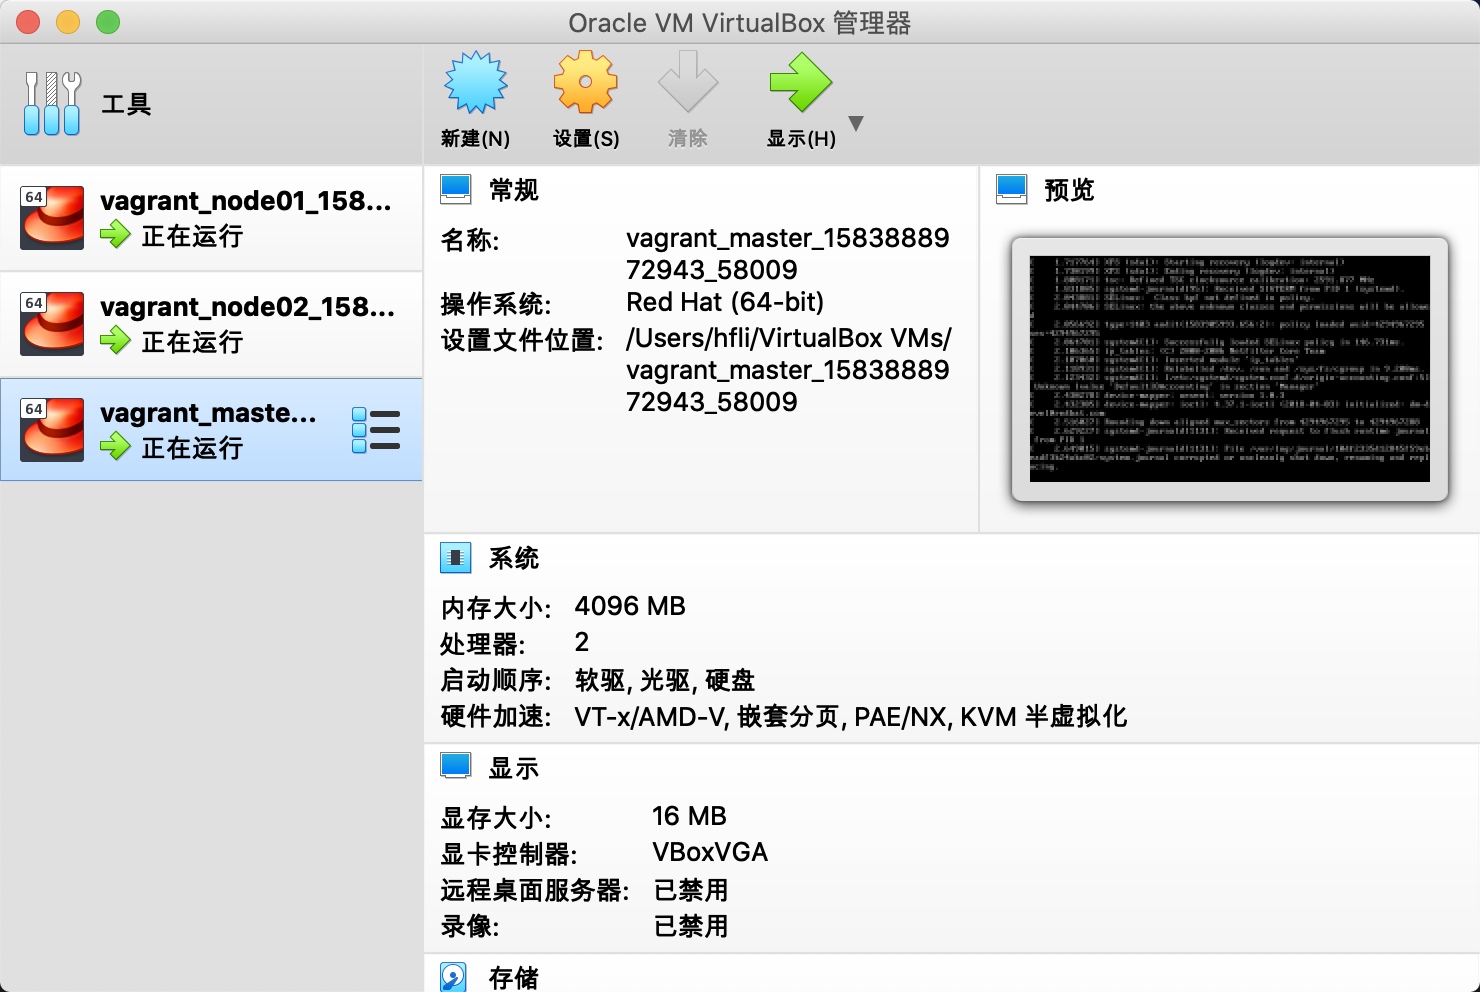
\includegraphics[keepaspectratio,alt={Virtualbox}]{images/Virtualbox-cluster.png}}
\caption{Virtualbox}
\end{figure}

这里master的域名配置有个坑，那就是hostnamanger会会生成一个master.example.com的ip映射在hosts文件里面，但是这个文件开头还有127.0.0.1 指向 master.example.com，像这样：

\begin{Shaded}
\begin{Highlighting}[]
\DecValTok{127.0.0.1}       \VariableTok{master}\OperatorTok{.}\VariableTok{example}\OperatorTok{.}\VariableTok{com}      \VariableTok{master}
\DecValTok{127.0.0.1}   \VariableTok{localhost} \VariableTok{localhost}\OperatorTok{.}\VariableTok{localdomain} \VariableTok{localhost4} \VariableTok{localhost4}\OperatorTok{.}\VariableTok{localdomain4}
\OperatorTok{::}\DecValTok{1}         \VariableTok{localhost} \VariableTok{localhost}\OperatorTok{.}\VariableTok{localdomain} \VariableTok{localhost6} \VariableTok{localhost6}\OperatorTok{.}\VariableTok{localdomain6}

\OperatorTok{\#\#} \VariableTok{vagrant}\OperatorTok{{-}}\VariableTok{hostmanager}\OperatorTok{{-}}\VariableTok{start}
\DecValTok{192.168.11.102}  \VariableTok{node02}\OperatorTok{.}\VariableTok{example}\OperatorTok{.}\VariableTok{com}
\DecValTok{192.168.11.100}  \VariableTok{master}\OperatorTok{.}\VariableTok{example}\OperatorTok{.}\VariableTok{com}
\DecValTok{192.168.11.101}  \VariableTok{node01}\OperatorTok{.}\VariableTok{example}\OperatorTok{.}\VariableTok{com}
\OperatorTok{\#\#} \VariableTok{vagrant}\OperatorTok{{-}}\VariableTok{hostmanager}\OperatorTok{{-}}\ControlFlowTok{end}
\end{Highlighting}
\end{Shaded}

所以这里设置的\texttt{master.hostmanager.aliases}，同时要手动修改hostname：

\begin{Shaded}
\begin{Highlighting}[]
\ExtensionTok{hostnamectl}\NormalTok{ set{-}hostname master.example.com}
\end{Highlighting}
\end{Shaded}

\subsection{安装依赖项}\label{ux5b89ux88c5ux4f9dux8d56ux9879}

各个节点上都需要安装docker环境，使用下面的命令安装：

\begin{Shaded}
\begin{Highlighting}[]
\ExtensionTok{yum} \AttributeTok{{-}y}\NormalTok{ install docker{-}1.13.1}

\CommentTok{\# http://softpanorama.org/VM/Docker/Installation/rhel7\_docker\_package\_dockerroot\_problem.shtml}

\ExtensionTok{usermod} \AttributeTok{{-}aG}\NormalTok{ dockerroot vagrant}

\FunctionTok{cat} \OperatorTok{\textgreater{}}\NormalTok{ /etc/docker/daemon.json }\OperatorTok{\textless{}\textless{}EOF}
\StringTok{\{}
\StringTok{    "group": "dockerroot"}
\StringTok{\}}
\OperatorTok{EOF}

\ExtensionTok{systemctl}\NormalTok{ enable docker}
\ExtensionTok{systemctl}\NormalTok{ start docker}
\end{Highlighting}
\end{Shaded}

同时需要禁用掉SELinux：

\begin{Shaded}
\begin{Highlighting}[]
\ExtensionTok{setenforce}\NormalTok{ 0}
\FunctionTok{sed} \AttributeTok{{-}i} \StringTok{\textquotesingle{}s/SELINUX=enforcing/SELINUX=permissive/g\textquotesingle{}}\NormalTok{ /etc/selinux/config}
\end{Highlighting}
\end{Shaded}

而在master上需要装更多的依赖项：

\begin{Shaded}
\begin{Highlighting}[]
\ExtensionTok{yum}\NormalTok{ install wget git net{-}tools bind{-}utils yum{-}utils iptables{-}services bridge{-}utils bash{-}completion kexec{-}tools sos psacct}

\ExtensionTok{yum}\NormalTok{ install unzip}

\ExtensionTok{yum} \AttributeTok{{-}y}\NormalTok{ install https://releases.ansible.com/ansible/rpm/release/epel{-}7{-}x86\_64/ansible{-}2.9.6{-}1.el7.ans.noarch.rpm}
\end{Highlighting}
\end{Shaded}

这里安装依赖项之前，可以考虑将Base源替换为163源，这样速度会稍微快一点。

\subsection{配置ssh访问}\label{ux914dux7f6esshux8bbfux95ee}

应为整个集群安装是在master上进行的，但实际上有一些东西是需要操作node的，因此要配置好在master上能直接无密码登录到其他的node上。这里通过ssh私钥的形式来设置，首先在Vagrantfile中:

\begin{Shaded}
\begin{Highlighting}[]
\ControlFlowTok{if} \VariableTok{File}\OperatorTok{.}\VariableTok{exist}\NormalTok{?}\OperatorTok{(}\StringTok{".vagrant/machines/master/virtualbox/private\_key"}\OperatorTok{)}
    \VariableTok{master}\OperatorTok{.}\VariableTok{vm}\OperatorTok{.}\NormalTok{provision }\StringTok{"master{-}key"}\OperatorTok{,} \FunctionTok{type}\OperatorTok{:} \StringTok{"file"}\OperatorTok{,} \VariableTok{source}\OperatorTok{:} \StringTok{".vagrant/machines/master/virtualbox/private\_key"}\OperatorTok{,} \VariableTok{destination}\OperatorTok{:} \StringTok{"/home/vagrant/.ssh/master.key"}
\ControlFlowTok{end}
\ControlFlowTok{if} \VariableTok{File}\OperatorTok{.}\VariableTok{exist}\NormalTok{?}\OperatorTok{(}\StringTok{".vagrant/machines/node01/virtualbox/private\_key"}\OperatorTok{)}
    \VariableTok{master}\OperatorTok{.}\VariableTok{vm}\OperatorTok{.}\NormalTok{provision }\StringTok{"node01{-}key"}\OperatorTok{,} \FunctionTok{type}\OperatorTok{:} \StringTok{"file"}\OperatorTok{,} \VariableTok{source}\OperatorTok{:} \StringTok{".vagrant/machines/node01/virtualbox/private\_key"}\OperatorTok{,} \VariableTok{destination}\OperatorTok{:} \StringTok{"/home/vagrant/.ssh/node01.key"}
\ControlFlowTok{end}
\ControlFlowTok{if} \VariableTok{File}\OperatorTok{.}\VariableTok{exist}\NormalTok{?}\OperatorTok{(}\StringTok{".vagrant/machines/node02/virtualbox/private\_key"}\OperatorTok{)}
    \VariableTok{master}\OperatorTok{.}\VariableTok{vm}\OperatorTok{.}\NormalTok{provision }\StringTok{"node02{-}key"}\OperatorTok{,} \FunctionTok{type}\OperatorTok{:} \StringTok{"file"}\OperatorTok{,} \VariableTok{source}\OperatorTok{:} \StringTok{".vagrant/machines/node02/virtualbox/private\_key"}\OperatorTok{,} \VariableTok{destination}\OperatorTok{:} \StringTok{"/home/vagrant/.ssh/node02.key"}
\ControlFlowTok{end}
\end{Highlighting}
\end{Shaded}

然后通过下面的命令将文件拷贝过去：

\begin{Shaded}
\begin{Highlighting}[]
\ExtensionTok{vagrant}\NormalTok{ provision }\AttributeTok{{-}{-}provision{-}with}\NormalTok{ master{-}key,node01{-}key,node02{-}key}
\end{Highlighting}
\end{Shaded}

这一步的目的是因为Vagrant在创建这些node的时候，这个key还没有生成，只能在创建完之后才能成功拷贝过去。然后设置master的ssh配置：

\begin{Shaded}
\begin{Highlighting}[]
\CommentTok{\# vagrant ssh master}
\CommentTok{\#vim \textasciitilde{}/.ssh/config}
\ExtensionTok{Host} \PreprocessorTok{*}
\ExtensionTok{StrictHostKeyChecking}\NormalTok{ no}
\end{Highlighting}
\end{Shaded}

到这一步，docker、ssh访问都应该是成功的，如果想检查是否配置成功，可以在master上测试：

\begin{Shaded}
\begin{Highlighting}[]
\ExtensionTok{vagrant}\NormalTok{ ssh master}
\ExtensionTok{docker} \AttributeTok{{-}v}
\FunctionTok{ssh} \AttributeTok{{-}i}\NormalTok{ node01.key vagrant@node01.example.com}
\end{Highlighting}
\end{Shaded}

\subsection{创建Inventory}\label{ux521bux5efainventory}

通过ansible执行需要一个hosts文件，如下：

\begin{Shaded}
\begin{Highlighting}[]
\KeywordTok{[OSEv3:children]}
\DataTypeTok{masters}
\DataTypeTok{nodes}
\DataTypeTok{etcd}

\KeywordTok{[OSEv3:vars]}
\DataTypeTok{ansible\_ssh\_user}\OtherTok{=}\StringTok{vagrant}
\DataTypeTok{ansible\_become}\OtherTok{=}\KeywordTok{true}
\DataTypeTok{openshift\_deployment\_type}\OtherTok{=}\StringTok{origin}
\DataTypeTok{openshift\_disable\_check}\OtherTok{=}\StringTok{disk\_availability,memory\_availability,docker\_storage,docker\_image\_availability}

\KeywordTok{[masters]}
\DataTypeTok{master.example.com ansible\_ssh\_private\_key\_file}\OtherTok{=}\StringTok{"/home/vagrant/.ssh/master.key"}

\KeywordTok{[etcd]}
\DataTypeTok{master.example.com ansible\_ssh\_private\_key\_file}\OtherTok{=}\StringTok{"/home/vagrant/.ssh/master.key"}

\KeywordTok{[nodes]}
\DataTypeTok{master.example.com containerized}\OtherTok{=}\StringTok{false etcd\_ip=192.168.11.100 openshift\_node\_group\_name=\textquotesingle{}node{-}config{-}master{-}infra\textquotesingle{}  ansible\_ssh\_private\_key\_file="/home/vagrant/.ssh/master.key"}
\DataTypeTok{node01.example.com openshift\_node\_group\_name}\OtherTok{=}\StringTok{\textquotesingle{}node{-}config{-}compute\textquotesingle{} ansible\_ssh\_private\_key\_file="/home/vagrant/.ssh/node01.key"}
\DataTypeTok{node02.example.com openshift\_node\_group\_name}\OtherTok{=}\StringTok{\textquotesingle{}node{-}config{-}compute\textquotesingle{} ansible\_ssh\_private\_key\_file="/home/vagrant/.ssh/node02.key"}
\end{Highlighting}
\end{Shaded}

这里有几点坑： * \texttt{containerized=false\ etcd\_ip=192.168.11.100}这个如果不加会导致\href{https://github.com/eliu/openshift-vagrant/issues/10}{``Wait for control plane pods to appear''}错误

这个文件保存到/etc/ansible/hosts。

\subsection{安装}\label{ux5b89ux88c5}

在master上面安装ansible:

\begin{Shaded}
\begin{Highlighting}[]
\ExtensionTok{yum} \AttributeTok{{-}y}\NormalTok{ install https://releases.ansible.com/ansible/rpm/release/epel{-}7{-}x86\_64/ansible{-}2.9.6{-}1.el7.ans.noarch.rpm}
\FunctionTok{wget}\NormalTok{ https://github.com/openshift/openshift{-}ansible/archive/openshift{-}ansible{-}3.11.187{-}1.zip}
\end{Highlighting}
\end{Shaded}

然后，最好把openshift-ansible里面的mirror修改成国内的，否则很可能安装不成功或者要花很长时间：

\begin{Shaded}
\begin{Highlighting}[]
\FunctionTok{sed} \AttributeTok{{-}i} \StringTok{\textquotesingle{}s/mirror.centos.org/mirrors.163.com/g\textquotesingle{}}\NormalTok{ openshift{-}ansible/roles/openshift\_repos/templates/CentOS{-}OpenShift{-}Origin311.repo.j2}
\end{Highlighting}
\end{Shaded}

正是安装：

\begin{Shaded}
\begin{Highlighting}[]
\ExtensionTok{ansible{-}playbook}\NormalTok{ /home/vagrant/openshift{-}ansible/playbooks/prerequisites.yml }\KeywordTok{\&\&} \ExtensionTok{ansible{-}playbook}\NormalTok{ /home/vagrant/openshift{-}ansible/playbooks/deploy\_cluster.yml}
\end{Highlighting}
\end{Shaded}

如果一切正常的话，就可以安装成功了。其中有几步比较耗时(大概十分钟左右），需要点耐心：

\begin{verbatim}
TASK [openshift_node : Install node, clients, and conntrack packages]
TASK [openshift_node : Check status of node image pre-pull]
\end{verbatim}

成功之后，可以看到log：

\begin{verbatim}
PLAY RECAP ***********************************************************************************************************
localhost                  : ok=11   changed=0    unreachable=0    failed=0    skipped=5    rescued=0    ignored=0
master.example.com         : ok=622  changed=275  unreachable=0    failed=0    skipped=987  rescued=0    ignored=0
node01.example.com         : ok=130  changed=63   unreachable=0    failed=0    skipped=167  rescued=0    ignored=0
node02.example.com         : ok=130  changed=63   unreachable=0    failed=0    skipped=167  rescued=0    ignored=0


INSTALLER STATUS *****************************************************************************************************
Initialization               : Complete (0:00:18)
Health Check                 : Complete (0:00:04)
Node Bootstrap Preparation   : Complete (0:34:23)
etcd Install                 : Complete (0:00:32)
Master Install               : Complete (0:07:48)
Master Additional Install    : Complete (0:00:34)
Node Join                    : Complete (0:06:56)
Hosted Install               : Complete (0:00:56)
Cluster Monitoring Operator  : Complete (0:02:47)
Web Console Install          : Complete (0:01:45)
Console Install              : Complete (0:01:21)
Service Catalog Install      : Complete (0:07:53)
\end{verbatim}

然后就可以访问\texttt{https://master.example.com:8443/}了：

\begin{figure}
\centering
\pandocbounded{
\includegraphics[keepaspectratio,alt={Openshift home}]{images/Openshift-welcome.png}}
\caption{Openshift home}
\end{figure}

Reference: * \href{https://blog.csdn.net/sun_qiangwei/article/details/80443943}{OpenShift 3.9 多节点集群（Ansible）安装}


\end{document}
